\chapter{Problem definition and 3D-stacked integrated circuit model}
\label{cha:model}

\begin{summary}
\lipsum[1]
\end{summary}

\section{Introduction}
In Chapter \ref{cha:rol.icdesign}, we have presented a review of the literature about the field of microelectronics design. We have highlighted some limitations of the current tools that already occur for 2D-ICs. In this chapter, we will define the 3D floorplanning problem, which is the issue we tackle and show how we model it in order to propose improvements to design flows.

\section{Problem definition}
As stated in Chapter \ref{cha:rol.icdesign}, the limitations of the current design flows can be summarized in three points:
\begin{itemize}
\item Limitation of the design space exploration
\item Unicriterion optimization or trade-off analysis on a limited number of criteria
\item Few 3D-SIC dedicated tools
\end{itemize}
In order to address these limitations, we propose in this thesis a methodology based on multi-objective/criteria tools and taking into account 3D-SIC specificities to explore of the design space.

While this methodology could be applied at different levels in a design flow, we have focused our development in the logical design step and the virtual prototyping flow, more specifically the floorplanning with performance assessments.

\subsection{Design an IC}
In order to meet the specifications, a design has to first make choice at a physical level:
\begin{itemize}
\item Targeted architecture, e.g. ASIC, FPGA
\item Number of functional units
\item Number of memories and their size
\item The general layout
\item ...
\end{itemize}
Since the 3D-SICs are based on conventional circuits, the options and degrees of freedom coming from 2D-ICs are still present:
\begin{itemize}
\item Process technology, e.g. 180 nm to 22 nm CMOS
\item Memories technology, e.g. SRAM, DRAM, FLASH
\item Communication infrastructure, e.g. bus, Network-on-Chip
\item ...
\end{itemize}
In addition to those options and degrees of freedom coming from 2D-ICs, there are also numerous 3D-SIC's parameters \cite{659500}:
\begin{itemize}
\item Number of tiers to use
\item Place and route of the functional units between the tiers
\item Technology to use per tiers (heterogeneity)
\item Interconnection and geometry between tiers
\item 3D-SIC integration technology
\item 3D-SIC assembly technology
\item ...
\end{itemize}

The above mentioned parameters illustrate the numerous possibilities for designing a circuit and how the design space for 2D-ICs becomes much bigger when considering 3D-SICs. The main issue is therefore to choose the most efficient combination among all those options. This can thus be compared to a combinatorial optimization problem. Also, given the multi-criteria nature of designing 3D-SIC, we choose to take into account all the criteria simultaneously for the optimization. In our case, due to the heterogeneous nature of the criteria (see Section \ref{sec:crit}), we have few hopes to successfully adopt an exact method and we will therefore use metaheuristics which are commonly-used tools for such kinds of problems. In the next section will define the criteria that a designer can consider.

\section{Model and criteria definition}
\label{sec:crit}

Typically, the criteria that have to be optimized simultaneously can be the performance, the power consumption, the cost, the package size, the heat dissipation, etc. In this model, we will define five criteria which are among the most important parameters while designing a circuit~\cite{DBLP:conf/3dic/MilojevicCCRRSAPM09}:
\begin{enumerate}
\item \textit{The interconnection global length}: this parameter can reflect the global performance of a system. The objective is to minimize it in order to have, for instance, a short delay and low power consumption. It will be calculated using the Manhattan distance \cite{mandist06}:
\begin{equation}
d_{i,j}=|x_i-x_j|+|y_i-y_j|
\end{equation}
where $(x_k, y_k)$ is the geometrical coordinates of the $k^{th}$ block. As a first approximation, the center point of each block will be selected as reference coordinate. Also, since it is more interesting to place close to each other two blocks that require a large bandwidth ($BW$) to communicate, we will balance the values as follows:
\begin{equation}
d_{i,j}'=\frac{d_{i,j}}{BW_{ij}}
\end{equation}
where $BW_{ij}$ is the bandwidth required between the block $i$ and the block $j$. The global interconnection length $D$ will be the sum of $d_{i,j}'$ for all communicating blocks:
\begin{equation}
D=\sum d'_{i,j}
\end{equation}
\item \textit{The cost}: an economical factor is obviously an important criteria for a design. This criteria has been estimated with the aid of an expert in 3D-SIC manufacturing. While a circuit can be more efficient with many layers, it will also be more expensive. This criteria has to be minimized. Due to the confidential nature of the cost of a 3D-SIC, we will consider a simplified model where the cost is proportional to the area and increasing exponentially with the number of tiers:
\begin{equation}
cost=a(tech).S+b(tech)^{layer~number}
\label{eqn:cost}
\end{equation}
where $a(tech)$ and $b(tech)$ are coefficient depending on the technology assigned.
Let us note that this criterion includes both discrete and continuous variables.
\item \textit{The package volume}: this can be an important criteria when designing embedded circuits. The package volume is calculated as follows:
\begin{equation}
volume=largest~layer~size~*~stack~thickness~*~number~of~tiers
\label{eqn:volume}
\end{equation}
A large appoximation of 200 $\mu$m will be made for the thickness of one tiers.
Let us note that this criterion includes both discrete (number of tiers) and continuous variables (layer size).
\item \textit{The clock tree position}: in this model, we consider a synchronous system so the objective is to minimize the distance between each block and the clock tree in order to have a high frequency. We choose arbitrarily to approximate the reference point as a fixed point located at the upper left corner of the middle tier of the 3D-SIC.
% Another solution being worked on is to determine the best position for the clock tree for a given floorplan.
\item \textit{The thermal dissipation}: thermal dissipation is one of the major issues when designing 3D-SICs. It can be more appropriate to place two blocks underneath each other in successive tiers but a high heat dissipation may happen in intensive computational process. This criterion is a research topic on its own \cite{1112292, 1486402}. Here we will use a simplified evaluation model with finite elements. This model will consider that the dissipated power, intra- or inter- tiers, is inversely proportional to the distance to the heat source:
\begin{equation}
P_{diss} = P_{comp} \sum_{i=1}^{n} \frac{1}{R_{th, i} \cdot r}
\label{eqn:pdiss}
\end{equation}
where $r$ the distance to the heat source and $R_{th, i}$ the thermal resistance depending on whether the dissipation is intra- or inter- tiers.
This criteria is still on early development stage and we can generate thermal maps of a floorplan as shown in Fig. \ref{fig:thermalmap} but this is currently based on finite elements \cite{4263187} which require quite a long computational time even for a simplified thermal model.
This criterion in its current development stage is difficult to integrate to the exploration process, due to the computation time of finite elements methods. In the current work, we will simply compute the peak power of a circuit which can be done more quickly.

\begin{figure}[h!]
\begin{center}
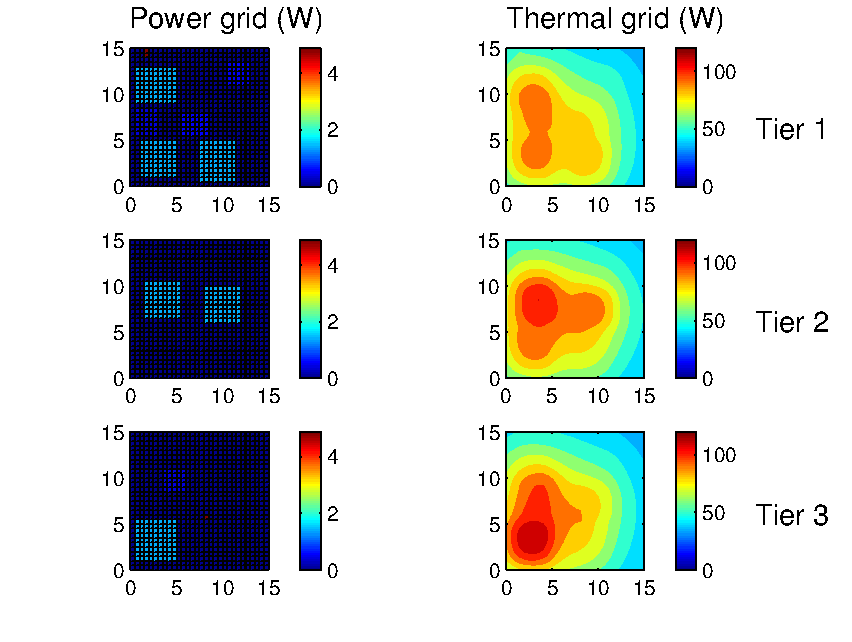
\includegraphics[width=1\linewidth]{heatmapex_gray2.pdf}
\end{center}
\vspace{-0.5cm}
\caption{Power grid and thermal map of a floorplan (3 tiers)}
\label{fig:thermalmap}
\end{figure}

%\item \textit{The power consumption}: the objective is to minimize the power consumption which can be a crucial criterion for embedded systems. Generally, the power consumption can be defined as the sum of a static ($P_{stat}$) (given data from the component datasheet) and a dynamic ($P_{dyn}$) consumption:
%\begin{equation}
%P=P_{stat}+P_{dyn}
%\end{equation}
%\begin{equation}
%P_{stat}=[given~data]
%\end{equation}
%\begin{equation}
%P_{dyn}=\alpha.C.V_{dd}^2.f.[tech]
%\end{equation}
%where $\alpha$ represents the toggle rate, $C$ the capacitance, $V_{dd}$ the voltage, $f$ the frequency and $[tech]$ a rectification factor due to the technology assigned.
\end{enumerate}

At first, we will focus on the three first criteria in order to be able to have a visualization of the design space. We will also arbitrarily introduce some limitations in term of degrees of freedom to analyse what happens if we release a constraint. This will be done while considering the three same criteria, in order to keep a visualization and show how the flexibility of MOO will improve the information and the results. Then we will analyse our methodology with the five first criteria that have been presented. As stated, the sixth criterion is currently unused. Actually, it has been simulated and tested but we need data from the manufacturers which are not easily available.
%As for the thermal dissipation, simulations are possible (see Fig.~\ref{fig:thermalmap}) but due to its current development stage it is difficult to integrate it in the exploration process due to the computing time of finite elements.

\section{Design methodology}
In summary, the problem we are facing is to place several blocks that have to be assigned in many tiers while considering multiple conflicting criteria. Now that our model has been defined, we will present a proposition of a new design methodology based on multi-objective optimization.

As explained in Chapter \ref{cha:rol.icdesign}, designing ICs implies numerous choices and designers are likely to freeze a certain amount of choices on basis of their experience. This will therefore limit the exploration of the design space and good solutions may be ignored.

In order to enable an efficient design space exploration, we propose a method in four steps based on MCDA which is illustrated in Fig.~\ref{fig:mcdaflow}. The implementation will be briefly presented in the next section.

\begin{figure}[h!]
\begin{center}
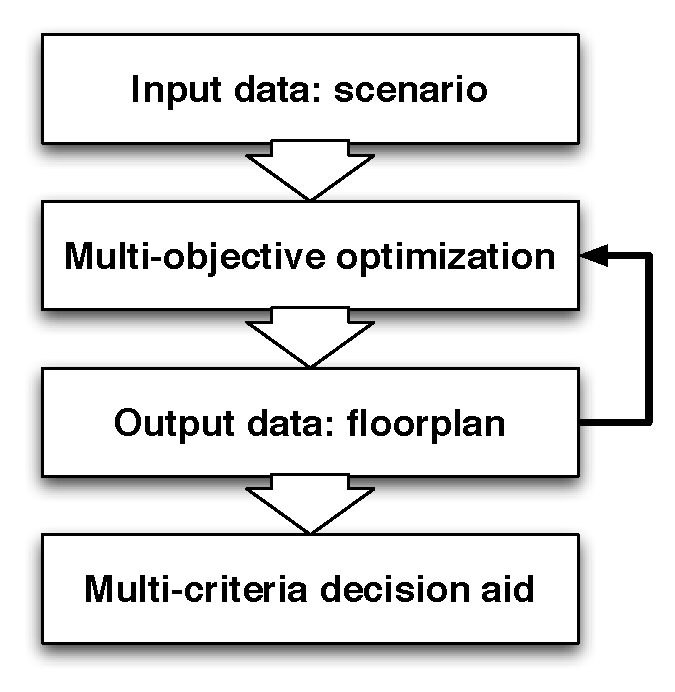
\includegraphics[width=0.5\linewidth]{MCDA_Method.pdf}
\end{center}
\vspace{-0.5cm}
\caption{MCDA-based design methodology for 3D DSE floorplanning}
\label{fig:mcdaflow}
\end{figure}

For the problem we consider, the input data will contain the information about the scenario:
\begin{itemize}
\item Type and number of blocks: computational units, memories, etc.
\item Size of the blocks: inherent to the block.
\item Minimum aspect ratio: we consider a degree of freedom where a block can have its dimensions varying within an aspect ratio range. This means that a block does not have to be square, as shown in Fig. \ref{fig:ff_ex}. This parameter can influence the delay in a block.
\item Size variability of a block: we add this degree of freedom considering that the specified size of a block can be fixed by the designer but this fixed size can restrict the design space exploration. The variability of a block's size can have effect on the performances and the global footprint.
\end{itemize}
In addition, the bandwidth requirements are needed as they will indicate which are the important interconnections and prevent two blocks that require a large bandwidth from being too far from each other. The available manufacturing technologies are also useful to enable the design of heterogeneous systems.

\begin{figure}[h!]
\begin{center}
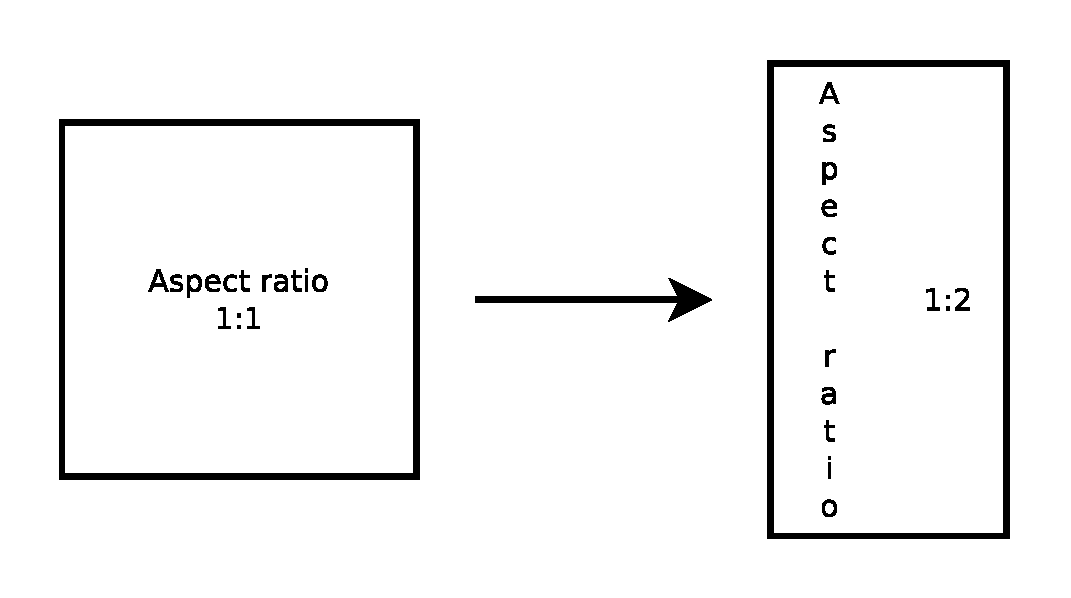
\includegraphics[width=0.6\linewidth]{form_factor_ex.pdf}
\end{center}
\vspace{-0.5cm}
\caption{Example of aspect ratio degree of freedom}
\label{fig:ff_ex}
\end{figure}

The combination of all the parameters described in the model are the possible alternatives for a 3D-SIC design and will provide output data after design space exploration. For a floorplanning problem the required output data are generally the geometrical layout of the circuit~\cite{DBLP:conf/3dic/MilojevicCCRRSAPM09}:
\begin{itemize}
\item The geometrical coordinates for each block and the assigned layer.
\item The size of each block (if it can vary from the specified size).
\item The aspect ratio for each block.
\item The technology assigned to each tier: this will reduce the size of each block. The size of a block will define the number of transistors inside using a given technology, for example 180 nm. For a constant number of transistors, if the block is manufactured with a smaller technology, let us say 45 nm, then its size will be divided by a (180/45)$^2$ factor, as shown in Fig.~\ref{fig:tech_ex}. Please note, that this factor is a rough approximation which is not always met with real physical design.
\end{itemize}

\begin{figure}[h!]
\begin{center}
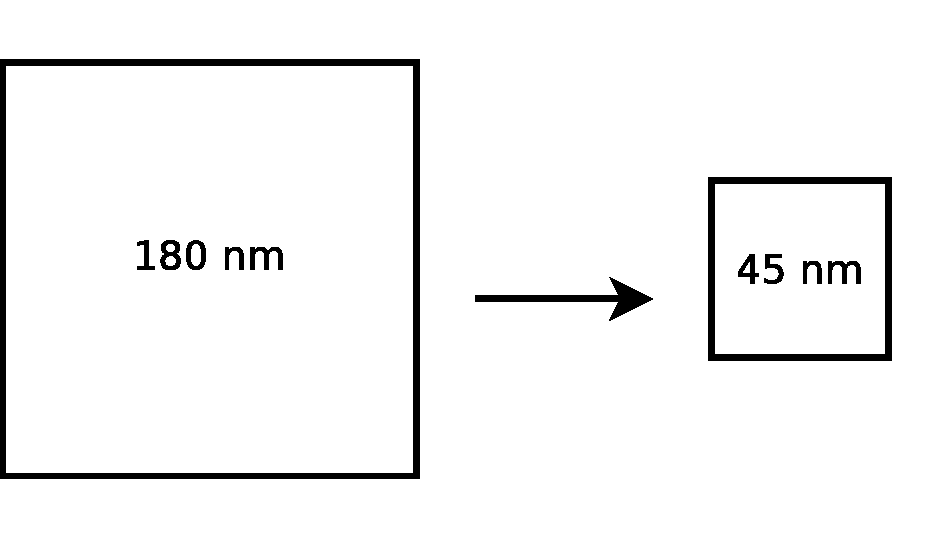
\includegraphics[width=0.5\linewidth]{tech_ex.pdf}
\end{center}
\vspace{-0.5cm}
\caption{The use of different manufacturing technologies results in a size variation}
\label{fig:tech_ex}
\end{figure}

\section{Case study and implementation}
In this section, we will briefly explain the implementation of our design method and show some experimental results based on this first approach. Due to the huge size of the design space, an explicit enumeration of the possible solutions will take considerable time. We will therefore apply a metaheuristic and more specifically a NSGA-II algorithm. We consider a case study based on the 3MF MPSoC platform developed at IMEC~\cite{dmilojev08b}.
%This case study has been implemented using Matlab and all data were coded using matrices.

\subsection{Description of the case study and modeling}
The 3MF MPSoC is made of 13 blocks as shown on Fig. \ref{fig:imec3mf}:
\begin{itemize}
\item 6 ADRES processors (\cite{conf/fpl/VeredasSMM05})
\item 2 data memories (L2D\#)
\item 2 instruction memories (L2Is\#)
\item 1 external memory interface (EMIF)
\item 1 input/output processor (FIFO)
\item 1 ARM processor (ARM)
\end{itemize}
Details about the area required for each component is given in Table \ref{tab:scenarmat} for a 90 nm technology. This table is also the input matrix required to specify the scenario.

\begin{table*}[pt!]
\caption{Scenario input matrix example}
\begin{center}
\begin{scriptsize}
\begin{tabular}{|c|c|c|c|c|}
\hline Component & ID & Size (90 nm) & Min aspect ratio & Size variability\\
\hline ADRES 1\texttildelow 6 & 1\texttildelow 6 & 18.6 mm$^2$ & 0.5 & 0.1\\
FIFO & 7 & 0.54 mm$^2$ & 0.5 & 0.1\\
L2D1-2 & 8-9 & 6.74 mm$^2$ & 0.5 & 0.1\\
L2Is1-2 & 10-11 & 6.62 mm$^2$ & 0.5 & 0.1\\
EMIF & 12 & 0.66 mm$^2$ & 0.5 & 0.1\\
ARM & 13 & 0.89 mm$^2$ & 0.5 & 0.1\\
\hline
\end{tabular}
\end{scriptsize}
\end{center}
\begin{center}
ID: Component identification number
\end{center}
\label{tab:scenarmat}
\end{table*}

\begin{figure}[h!]
\begin{center}
%\includegraphics[width=7cm]{imec3mf.png}
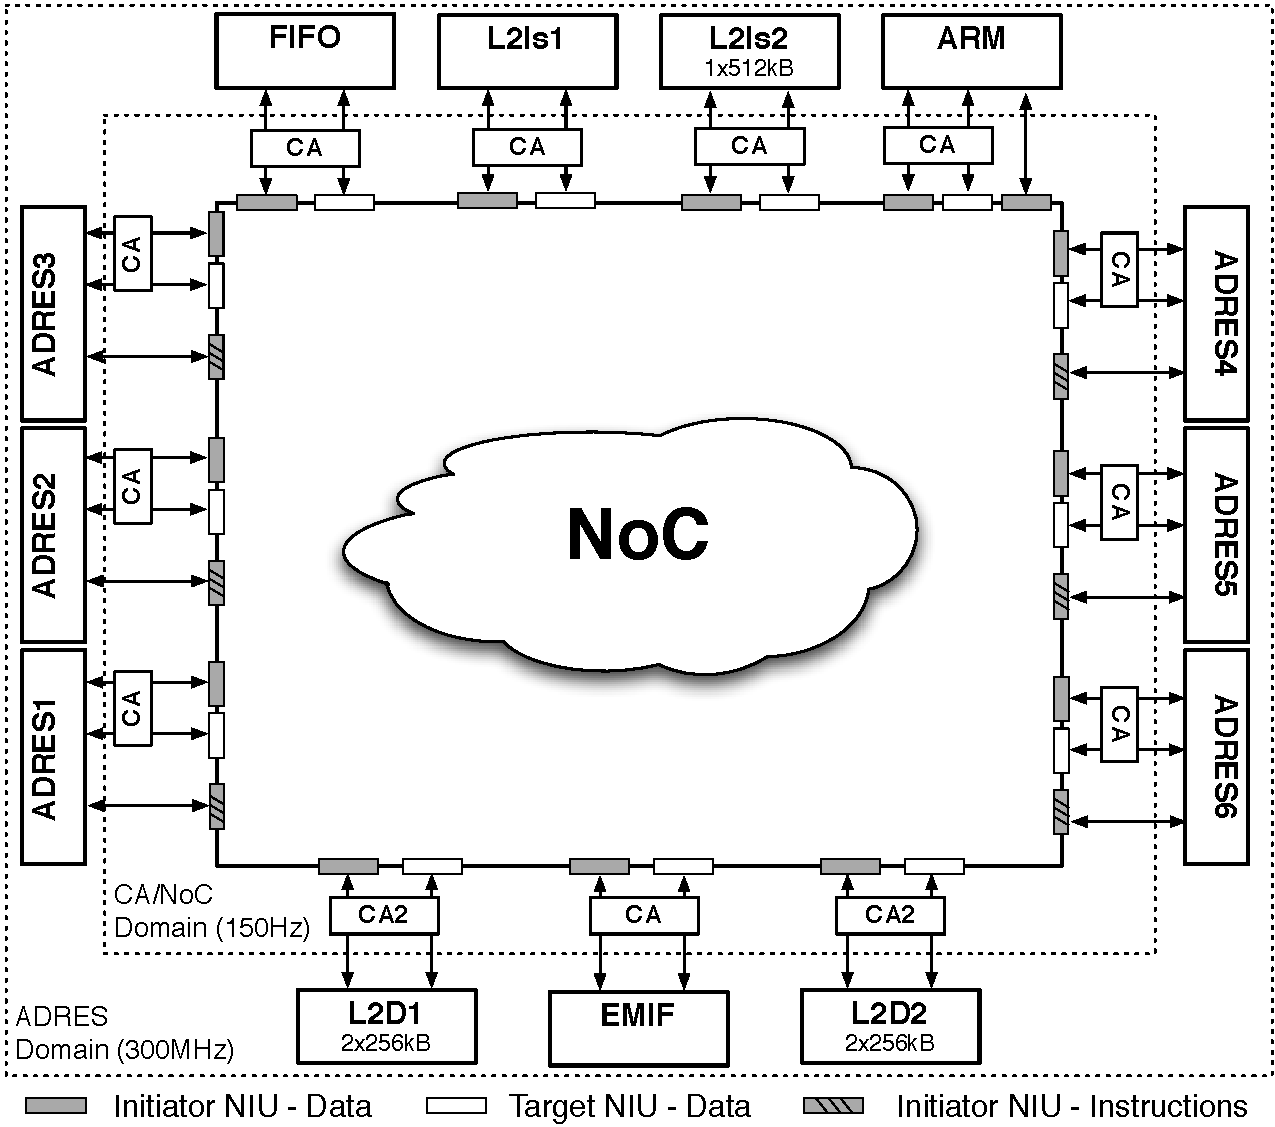
\includegraphics[width=7cm]{3MFMPSoC.pdf}
\end{center}
\vspace{-0.3cm}
\caption{Architecture of the 3MF MPSoC platform~\cite{dmilojev08b}}
\label{fig:imec3mf}
\end{figure}

The 3MF MPSoC can be configured for three use cases which have specific bandwidth requirements. For the following results, we will base our simulation on the "data split scenario" configuration which possesses the communication specifications shown in Table \ref{tab:3mfbw}. This information is implemented, as shown in Table \ref{tab:bwmatrix}, in an input matrix which is built by specifying the communication structure: the first column will contain the ID of the source block and each next pairs of columns will contain the ID of the target blocks and the bandwidth required.

\begin{table*}[pt!]
\caption{"Data split scenario" bandwidth requirements}
\begin{center}
\begin{scriptsize}
\begin{tabular}{|c|c|c|}
\hline Source & Target & Bandwidth (MB/s)\\
\hline FIFO & EMIF & 39.6\\
EMIF & ADRES$i$ & 6.6\\
L2D1 & ADRES$i$ & 26.4\\
L2D2 & L2D1 & 52.7\\
ADRES$i$ & FIFO & 1.2\\
ADRES$i$ & L2D2 & 6.6\\
ADRES$j$ & L2Is1 & 300\\
ADRES$k$ & L2Is2 & 300\\
\hline
\end{tabular}
\end{scriptsize}
\end{center}
\begin{center}
Index: $i, j, k \in \mathbb{N}^{+};$\\
$1 \leq i \leq 6; 1\leq j \leq 3; 4 \leq k \leq 6$
\end{center}
\label{tab:3mfbw}
\end{table*}

The input data are thus shown in Tables \ref{tab:scenarmat} and \ref{tab:bwmatrix}. The available technologies are also needed to take advantage of the heterogeneity. An example matrix for this input data is given in Table \ref{tab:tech}. Since no information is given about the ARM unit bandwidth usage, we will simplify our problem and not include it in the implementation. We consider therefore 12 blocks to assign.

\begin{table*}[pt!]
\caption{Bandwidth input matrix}
\begin{center}
\begin{scriptsize}
\begin{tabular}{|c|c|c|c|c|c|c|c|c|c|c|c|c|}
\hline S & T & B & T & B & T & B & T & B & T & B & T & B \\
\hline 1 & 7 & 1.2 & 9 & 6.6 & 10 & 300 & 0 & 0 & 0 & 0 & 0 & 0\\
2 & 7 & 1.2 & 9 & 6.6 & 10 & 300 & 0 & 0 & 0 & 0 & 0 & 0\\
3 & 7 & 1.2 & 9 & 6.6 & 10 & 300 & 0 & 0 & 0 & 0 & 0 & 0\\
4 & 7 & 1.2 & 9 & 6.6 & 11 & 300 & 0 & 0 & 0 & 0 & 0 & 0\\
5 & 7 & 1.2 & 9 & 6.6 & 11 & 300 & 0 & 0 & 0 & 0 & 0 & 0\\
6 & 7 & 1.2 & 9 & 6.6 & 11 & 300 & 0 & 0 & 0 & 0 & 0 & 0\\
7 & 12 & 39.6 & 0 & 0 & 0 & 0 & 0 & 0 & 0 & 0 & 0 & 0\\
8 & 1 & 26.4 & 2 & 26.4 & 3 & 26.4 & 4 & 26.4 & 5 & 26.4 & 6 & 26.4\\
9 & 8 & 52.7 & 0 & 0 & 0 & 0 & 0 & 0 & 0 & 0 & 0 & 0\\
12 & 1 & 6.6 & 2 & 6.6 & 3 & 6.6 & 4 & 6.6 & 5 & 6.6 & 6 & 6.6\\
\hline
\end{tabular}
\end{scriptsize}
\end{center}
\begin{center}
S: source block ID\\
(T, B): target block ID and required bandwidth
\end{center}
\label{tab:bwmatrix}
\end{table*}

\begin{table}[p]
\caption{Available technologies input matrix example}
\begin{center}
\begin{tabular}{|c|c|c|c|c|}
\hline \multicolumn{5}{|c|}{Technology (nm)}\\
\hline 90 & 60 & 45 & 32 & 22\\
\hline
\end{tabular}
\end{center}
\label{tab:tech}
\end{table}

In summary, the problem we consider is to place 12 blocks while taking into account several criteria (5). We will also consider a scenario where the blocks can be placed on 1 up to 5 tiers. The input data will be processed to generate floorplans. Those output data will be encoded using the matrix model following the example shown in Table \ref{tab:outputmat}. They will be generated through a multi-objective optimization.

%\begin{table}[p]
%\caption{Output matrix template}
%\begin{center}
%\begin{scriptsize}
%\begin{tabular}{|c|c|c|c|c|c|c|c|c|}
%\hline ID & L & X & Y & S & AR & LX & LY & T\\
%\hline 1 & 2 & 4.5 & 6 & 18.6 & 1 & 4.3128 & 4.3128 & 90\\
%2 & 2 & 4 & 0.4 & 18.6 & 1 & 4.3128 & 4.3128 & 90\\
%3 & 3 & 3.1 & 6.9 & 18.6 & 1 & 4.3128 & 4.3128 & 90\\
%4 & 3 & 8.4 & 10.1 & 18.6 & 1 & 4.3128 & 4.3128 & 90\\
%5 & 3 & 6.6 & 2.2 & 18.6 & 1 & 4.3128 & 4.3128 & 90\\
%6 & 1 & 9 & 5.7 & 18.6 & 1 & 4.3128 & 4.3128 & 90\\
%7 & 1 & 10 & 3.5 & 0.54 & 1 & 0.7348 & 0.7348 & 90\\
%8 & 1 & 7.5 & 11 & 6.74 & 1 & 2.5962 & 2.5962 & 90\\
%9 & 2 & 9 & 5 & 6.74 & 1 & 2.5962 & 2.5962 & 90\\
%10 & 1 & 4.5 & 8 & 6.62 & 1 & 2.5729 & 2.5729 & 90\\
%11 & 2 & 8.6 & 0.4 & 6.62 & 1 & 2.5729 & 2.5729 & 90\\
%12 & 3 & 8.3 & 7.4 & 0.66 & 1 & 0.8124 & 0.8124 & 90\\
%\hline
%\end{tabular}
%\end{scriptsize}
%\end{center}
%\begin{center}
%\begin{scriptsize}
%ID: component identification number; L: assigned layer;\\
%(X, Y): geometrical coordinate; S: size (mm$^2$); AR: aspect ratio;\\
%(LX, LY): length in X and Y axis; T: assigned technology for the layer
%\end{scriptsize}
%\end{center}
%\label{tab:outputmat}
%\end{table}

%As explained earlier, the exploration process implies the issue of establishing the Pareto frontier. For that purpose, we choose to use NSGA-II~\cite{Deb00afast}. This algorithm allows the design space exploration as well as the establishment of the Pareto frontier at the same time. 
As explained earlier, we will use a metaheuristic to approximate the Pareto optimal frontier. For that purpose, we choose to use NSGA-II \cite{Deb00afast} as a proof of concept. The algorithm was run from a sample of 10~000 generated solutions from 1 up to 5 tiers. This size of random solutions is chosen arbitrarily since it is actually quite difficult to estimate the size of solution space, due to the heterogeneous nature of the criteria. Also, taking too few solutions (e.g. 100) is not interesting since we have empirically observed that our algorithm will take a longer time to begin to converge. 10~000 randomly-generated solutions seems to us a good compromise of time and workable solutions.
%As stated in Section 2, even for a really simplified problem, the solution space is huge (more than 10$^{18}$) so, taking 10~000, 100~000 or 1~000~000 randomly-generated solutions does not really imply any difference. 

%which makes us choose arbitrarily the number of random solutions for the first population of our algorithm.

In the following section, we will present some details about the implementation of the NSGA-II algorithm.

\subsection{Implementation of the exploration algorithm: NSGA-II}
As shown in Table \ref{tab:outputmat}, we choose to encode our data in real or integer values, so that they can be used directly by design tools:
\begin{itemize}
\item The component identification number (ID) is a fixed integer value linked to the component.
\item The assigned layer (L) is a discrete value ranging from 1 to 5 in the case study.
\item The geometrical coordinates (X,Y) are real values that depends on the dimension of the circuits and the aspect ratio of a block, so that the component cannot be placed outside the chip.
\item The size (S) is a fixed real value linked to the component.
\item The aspect ratio (AR) is a real value ranging from $AR_{min}$ to $1/AR_{min}$ where $AR_{min}$ is given as a specification as explained in Section 4.
\item The length in X and Y axis (LX, LY) are real values computed from the size and the aspect ratio.
\item The assigned technology per layer is a discrete value taking one of the specified technology (see Table \ref{tab:tech}).
\end{itemize}
This matrix will be our full chromosome for the NSGA-II algorithm (see example in Table \ref{tab:outputmat}.

\begin{table}[p]
\caption{Output matrix template}
\begin{center}
\begin{scriptsize}
\begin{tabular}{|c|c|c|c|c|c|c|c|c|}
\hline ID & L & X & Y & S & AR & LX & LY & T\\
\hline 1 & 2 & 4.5 & 6 & 18.6 & 1 & 4.3128 & 4.3128 & 90\\
2 & 2 & 4 & 0.4 & 18.6 & 1 & 4.3128 & 4.3128 & 90\\
3 & 3 & 3.1 & 6.9 & 18.6 & 1 & 4.3128 & 4.3128 & 90\\
4 & 3 & 8.4 & 10.1 & 18.6 & 1 & 4.3128 & 4.3128 & 90\\
5 & 3 & 6.6 & 2.2 & 18.6 & 1 & 4.3128 & 4.3128 & 90\\
6 & 1 & 9 & 5.7 & 18.6 & 1 & 4.3128 & 4.3128 & 90\\
7 & 1 & 10 & 3.5 & 0.54 & 1 & 0.7348 & 0.7348 & 90\\
8 & 1 & 7.5 & 11 & 6.74 & 1 & 2.5962 & 2.5962 & 90\\
9 & 2 & 9 & 5 & 6.74 & 1 & 2.5962 & 2.5962 & 90\\
10 & 1 & 4.5 & 8 & 6.62 & 1 & 2.5729 & 2.5729 & 90\\
11 & 2 & 8.6 & 0.4 & 6.62 & 1 & 2.5729 & 2.5729 & 90\\
12 & 3 & 8.3 & 7.4 & 0.66 & 1 & 0.8124 & 0.8124 & 90\\
\hline
\end{tabular}
\end{scriptsize}
\end{center}
\begin{center}
\begin{scriptsize}
ID: component identification number; L: assigned layer;\\
(X, Y): geometrical coordinate; S: size (mm$^2$); AR: aspect ratio;\\
(LX, LY): length in X and Y axis; T: assigned technology for the layer
\end{scriptsize}
\end{center}
\label{tab:outputmat}
\end{table}

We implemented our design space exploration following the steps of the NSGA-II which can be summarized by the diagram shown in Fig. \ref{fig:ga_steps}.

\begin{figure}[h!]
\begin{center}
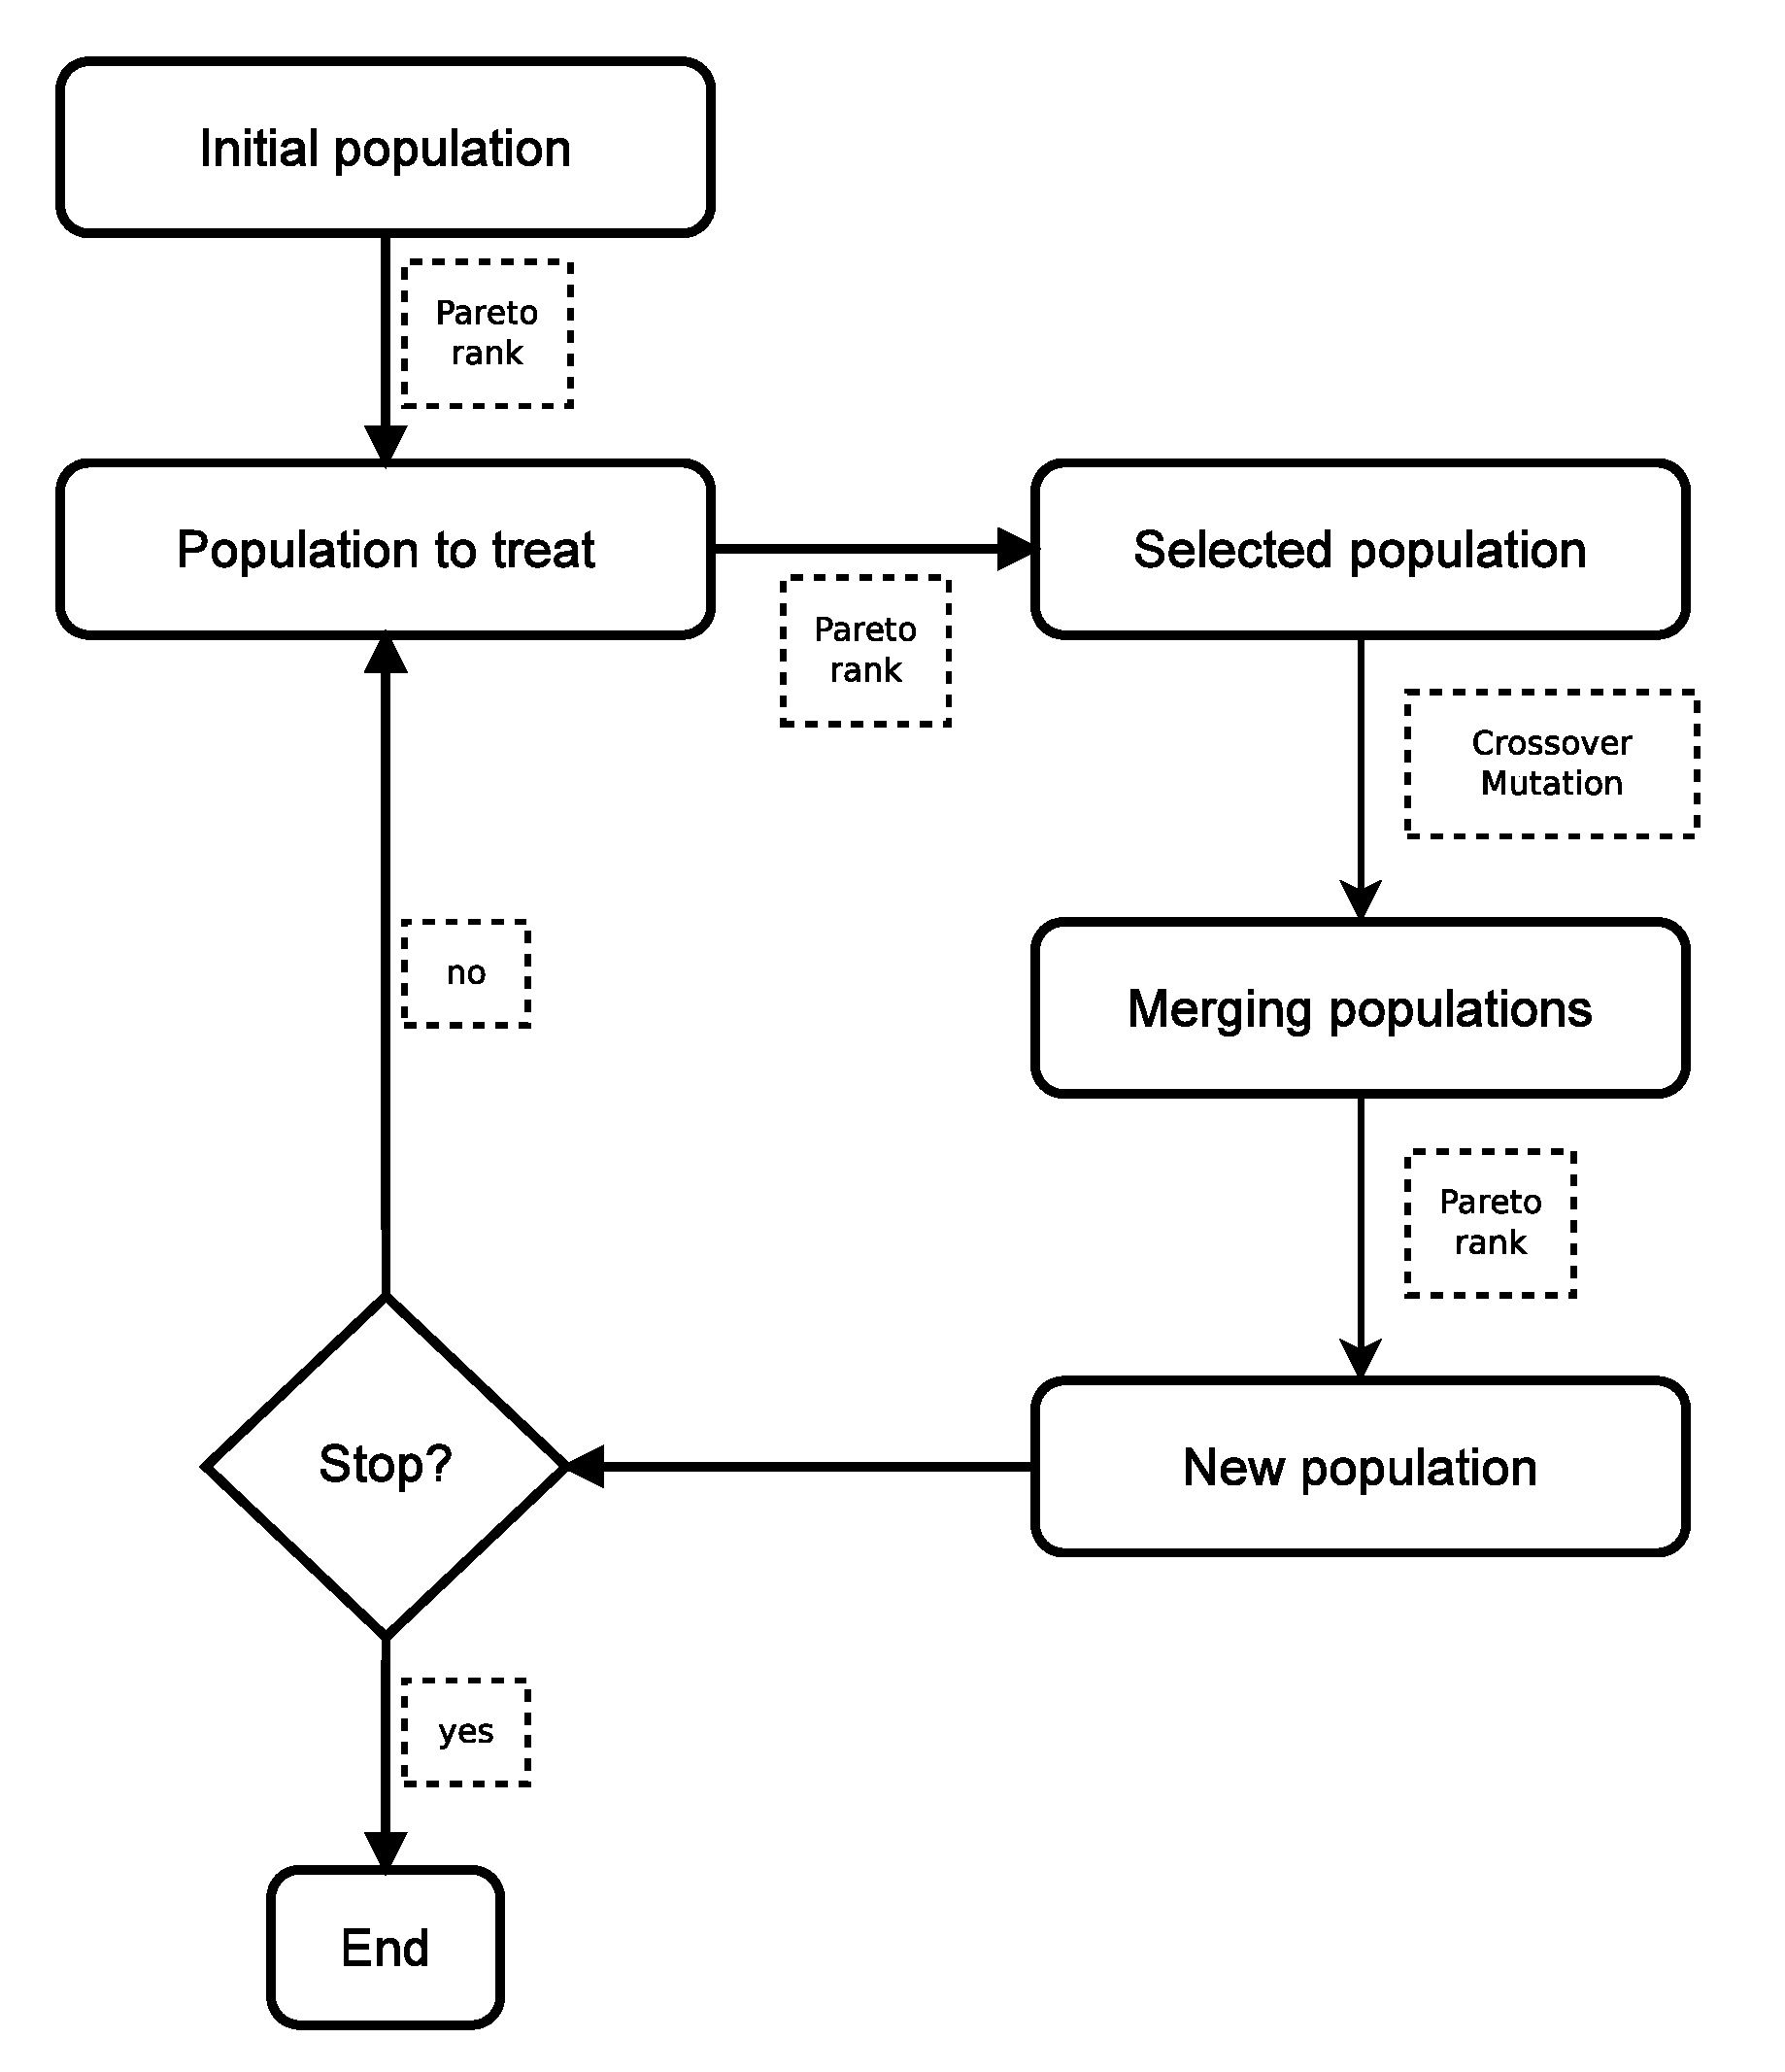
\includegraphics[width=7cm]{GA_dia_en.pdf}
\end{center}
\vspace{-0.5cm}
\caption{General NSGA-II steps}
\begin{center}
\end{center}
\label{fig:ga_steps}
\end{figure}

\subsubsection*{Initialization (the initial population)}
We will work with a minimum size of population, namely 50, which is a common value in GAs~\cite{Davis1989}. The initial population will be a set of at least 50 solutions with the best Pareto ranks from a randomly-generated set of 10~000 solutions. The produced set places the blocks randomly (using a uniform distribution) and does not allow overlapping between the blocks (these incorrect solutions are simply removed). We could of course use a greedy algorithm as well as a more advanced method such as GRASP (Greedy Randomized Adaptive Search Procedure)~\cite{HarSho87a}. This can be done as future work for comparison purposes.

Of course, having at least 50 Pareto solutions does not always happen. Actually, the selection is based on the Pareto rank so it does not include only the Pareto solutions (rank 1), but also the solutions with lower ranks until there are enough solutions.

\subsubsection*{Selection for crossover}
For the selection step, two solutions will be allowed to make a crossover depending on a roulette wheel where the probability is proportional to the normalized Euclidean distance between the solutions ordered by their Pareto rank in the objective space. The normalization is done as follows :
\begin{equation}
\frac{g_i(a_j)}{\max\limits_{a_j \in A} g_i(a_j)}
\end{equation}
where $A$ is the set of alternatives in the Pareto front with $a_j \in A$ and $g_i(a_j)$ is the evaluation of the alternative $a_j$ on the criterion $i$.

%As we want to ensure that our algorithm has intensification properties, we vary the crossover probability between two solutions according to their distance. In particular, we choose a crossover probability proportional to the Euclidean distance between the solutions, as shown in Fig. \ref{fig:cross_proba}. If two solutions are close to each other, they will have more chance to reproduce than if they are distant. This requires us to define a lower bound ($P_{c, min}$) and an upper bound ($P_{c, max}$) on the probabilities: $P_{c, min}$ is set for the solutions which are the furthest to each other while $P_{c, max}$ is set for those which are the closest. In between, the probability will vary linearly inside these bounds.

The probability for two solutions to do a crossover will vary linearly with the Euclidean distance between them, as shown in Fig. \ref{fig:cross_proba}. The distance between the two furthest alternatives ($d_furthest$) will be associated with a probability $P_{c, min}$ while the distance between the two closest alternatives ($d_closest$) will be associated with a probability $P_{c, max}$. If two solutions are close to each other, they will have more chance to reproduce than if they are distant. This is to ensure the intensification properties of our algorithm. Therefore, we will have to specify a lower bound ($P_{c, min}$) and an upper bound ($P_{c, max}$) for the crossover probability. $P_{c, min}$ is set for the solutions which are the furthest to each other while $P_{c, max}$ is set for those which are the closest. In between, the probability will vary linearly inside these bounds.

These values will be fixed as $[P_{c, min} = 0.6; P_{c, max} = 1.0]$ since these seem to be common values~\cite{Davis1989}.

\begin{figure}[h!]
\begin{center}
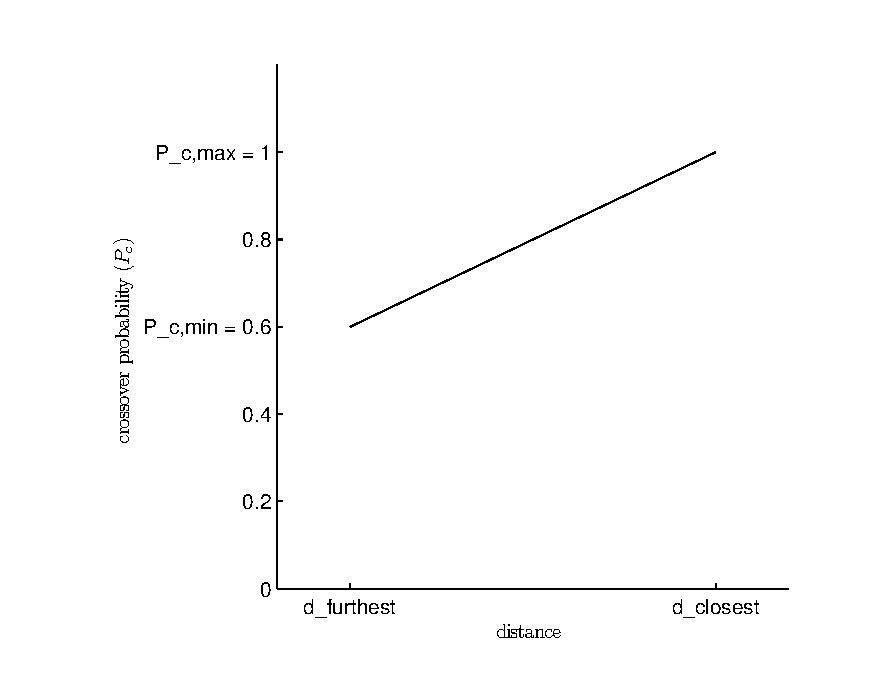
\includegraphics[width=8cm]{crossover_proba.eps}
\end{center}
\vspace{-0.5cm}
\caption{Evolution of the crossover probability as a function of the distance between two solutions}
\begin{center}
\end{center}
\label{fig:cross_proba}
\end{figure}

\subsubsection*{Crossover}

Let us now see how does the crossover occur. First, let us remark that it does not have limitations for the exploration process since the information contained in the matrix spans the whole circuit.

Second, we have to analyze how the chromosome is coded in order to see how we will apply the crossover step. For instance, let us choose the Layer (L) column as indicator for the crossover. If we order the matrix in Table \ref{tab:outputmat} following this column, we will have the Table \ref{tab:firstparentLrow} and the Table \ref{tab:secondparentLrow} for another solution that we will use for the crossover.

Now, without loss of generality, let us suppose that the crossover happens (randomly) on line 7. One of the child will be the Table \ref{tab:childLrow} and we see that the original scenario is not preserved since the first column (in bold) contains the same ID several times.

\begin{table}[pt]
\caption{First parent, ordered by L column; the line specifies the crossover cut}
\begin{center}
\begin{scriptsize}
\begin{tabular}{|c|c|c|c|c|c|c|c|c|}
\hline ID & L & X & Y & S & AR & LX & LY & T\\
\hline 6 & 1 & 9 & 5.7 & 18.6 & 1 & 4.3128 & 4.3128 & 90\\
7 & 1 & 10 & 3.5 & 0.54 & 1 & 0.7348 & 0.7348 & 90\\
8 & 1 & 7.5 & 11 & 6.74 & 1 & 2.5962 & 2.5962 & 90\\
10 & 1 & 4.5 & 8 & 6.62 & 1 & 2.5729 & 2.5729 & 90\\
1 & 2 & 4.5 & 6 & 18.6 & 1 & 4.3128 & 4.3128 & 90\\
2 & 2 & 4 & 0.4 & 18.6 & 1 & 4.3128 & 4.3128 & 90\\
9 & 2 & 9 & 5 & 6.74 & 1 & 2.5962 & 2.5962 & 90\\
\hline
\hline
11 & 2 & 8.6 & 0.4 & 6.62 & 1 & 2.5729 & 2.5729 & 90\\
3 & 3 & 3.1 & 6.9 & 18.6 & 1 & 4.3128 & 4.3128 & 90\\
4 & 3 & 8.4 & 10.1 & 18.6 & 1 & 4.3128 & 4.3128 & 90\\
5 & 3 & 6.6 & 2.2 & 18.6 & 1 & 4.3128 & 4.3128 & 90\\
12 & 3 & 8.3 & 7.4 & 0.66 & 1 & 0.8124 & 0.8124 & 90\\
\hline
\end{tabular}
\end{scriptsize}
\end{center}
\begin{center}
\begin{scriptsize}
ID: component identification number; L: assigned layer;\\
(X, Y): geometrical coordinate; S: size (mm$^2$); AR: aspect ratio;\\
(LX, LY): length in X and Y axis; T: assigned technology for the layer
\end{scriptsize}
\end{center}
\label{tab:firstparentLrow}
\end{table}

\begin{table}[pt]
\caption{Second parent, ordered by L column; the line specifies the crossover cut}
\begin{center}
\begin{scriptsize}
\begin{tabular}{|c|c|c|c|c|c|c|c|c|}
\hline ID & L & X & Y & S & AR & LX & LY & T\\
\hline 4 & 1 & 1.6 & 8.5 & 18.6 & 1 & 4.3128 & 4.3128 & 90\\
5 & 1 & 1.2 & 1.3 & 18.6 & 1 & 4.3128 & 4.3128 & 90\\
6 & 1 & 0.6 & 4.7 & 18.6 & 1 & 4.3128 & 4.3128 & 90\\
3 & 2 & 5.9 & 4 & 18.6 & 1 & 4.3128 & 4.3128 & 90\\
9 & 2 & 5.4 & 8 & 6.74 & 1 & 2.5962 & 2.5962 & 90\\
10 & 2 & 8.5 & 8.1 & 6.62 & 1 & 2.5729 & 2.5729 & 90\\
11 & 2 & 2.8 & 4.6 & 6.62 & 1 & 2.5729 & 2.5729 & 90\\
\hline
\hline
1 & 3 & 7 & 6.3 & 18.6 & 1 & 4.3128 & 4.3128 & 90\\
2 & 3 & 7.4 & 9.8 & 18.6 & 1 & 4.3128 & 4.3128 & 90\\
7 & 3 & 5.6 & 5.5 & 0.54 & 1 & 0.7348 & 0.7348 & 90\\
8 & 3 & 2.8 & 5.5 & 6.74 & 1 & 2.5962 & 2.5962 & 90\\
12 & 3 & 5.7 & 7.5 & 0.66 & 1 & 0.8124 & 0.8124 & 90\\
\hline
\end{tabular}
\end{scriptsize}
\end{center}
\begin{center}
\begin{scriptsize}
ID: component identification number; L: assigned layer;\\
(X, Y): geometrical coordinate; S: size (mm$^2$); AR: aspect ratio;\\
(LX, LY): length in X and Y axis; T: assigned technology for the layer
\end{scriptsize}
\end{center}
\label{tab:secondparentLrow}
\end{table}

\begin{table}[pt]
\caption{Possible child, ordered by L column}
\begin{center}
\begin{scriptsize}
\begin{tabular}{|c|c|c|c|c|c|c|c|c|}
\hline ID & L & X & Y & S & AR & LX & LY & T\\
\hline \textbf{6} & 1 & 9 & 5.7 & 18.6 & 1 & 4.3128 & 4.3128 & 90\\
\textbf{7} & 1 & 10 & 3.5 & 0.54 & 1 & 0.7348 & 0.7348 & 90\\
\textbf{8} & 1 & 7.5 & 11 & 6.74 & 1 & 2.5962 & 2.5962 & 90\\
\textbf{10} & 1 & 4.5 & 8 & 6.62 & 1 & 2.5729 & 2.5729 & 90\\
\textbf{1} & 2 & 4.5 & 6 & 18.6 & 1 & 4.3128 & 4.3128 & 90\\
\textbf{2} & 2 & 4 & 0.4 & 18.6 & 1 & 4.3128 & 4.3128 & 90\\
\textbf{9} & 2 & 9 & 5 & 6.74 & 1 & 2.5962 & 2.5962 & 90\\
\textbf{1} & 3 & 7 & 6.3 & 18.6 & 1 & 4.3128 & 4.3128 & 90\\
\textbf{2} & 3 & 7.4 & 9.8 & 18.6 & 1 & 4.3128 & 4.3128 & 90\\
\textbf{7} & 3 & 5.6 & 5.5 & 0.54 & 1 & 0.7348 & 0.7348 & 90\\
\textbf{8} & 3 & 2.8 & 5.5 & 6.74 & 1 & 2.5962 & 2.5962 & 90\\
\textbf{12} & 3 & 5.7 & 7.5 & 0.66 & 1 & 0.8124 & 0.8124 & 90\\
\hline
\end{tabular}
\end{scriptsize}
\end{center}
\begin{center}
\begin{scriptsize}
ID: component identification number; L: assigned layer;\\
(X, Y): geometrical coordinate; S: size (mm$^2$); AR: aspect ratio;\\
(LX, LY): length in X and Y axis; T: assigned technology for the layer
\end{scriptsize}
\end{center}
\label{tab:childLrow}
\end{table}

We observe that the only possible indicator for the crossover step is the ID column. Indeed if we order the two parents following the ID column, we have the Tables \ref{tab:firstparentIDrow} and \ref{tab:secondparentIDrow}. If we still consider that the crossover occurs on line 7, we can have the child shown in Table \ref{tab:childIDrow}. We see that there is no inconsistency since the scenario is still respected.

\begin{table}[pt]
\caption{First parent, ordered by ID column; the line specifies the crossover cut}
\begin{center}
\begin{scriptsize}
\begin{tabular}{|c|c|c|c|c|c|c|c|c|}
\hline ID & L & X & Y & S & AR & LX & LY & T\\
\hline 1 & 2 & 4.5 & 6 & 18.6 & 1 & 4.3128 & 4.3128 & 90\\
2 & 2 & 4 & 0.4 & 18.6 & 1 & 4.3128 & 4.3128 & 90\\
3 & 3 & 3.1 & 6.9 & 18.6 & 1 & 4.3128 & 4.3128 & 90\\
4 & 3 & 8.4 & 10.1 & 18.6 & 1 & 4.3128 & 4.3128 & 90\\
5 & 3 & 6.6 & 2.2 & 18.6 & 1 & 4.3128 & 4.3128 & 90\\
6 & 1 & 9 & 5.7 & 18.6 & 1 & 4.3128 & 4.3128 & 90\\
7 & 1 & 10 & 3.5 & 0.54 & 1 & 0.7348 & 0.7348 & 90\\
\hline
\hline
8 & 1 & 7.5 & 11 & 6.74 & 1 & 2.5962 & 2.5962 & 90\\
9 & 2 & 9 & 5 & 6.74 & 1 & 2.5962 & 2.5962 & 90\\
10 & 1 & 4.5 & 8 & 6.62 & 1 & 2.5729 & 2.5729 & 90\\
11 & 2 & 8.6 & 0.4 & 6.62 & 1 & 2.5729 & 2.5729 & 90\\
12 & 3 & 8.3 & 7.4 & 0.66 & 1 & 0.8124 & 0.8124 & 90\\
\hline
\end{tabular}
\end{scriptsize}
\end{center}
\begin{center}
\begin{scriptsize}
ID: component identification number; L: assigned layer;\\
(X, Y): geometrical coordinate; S: size (mm$^2$); AR: aspect ratio;\\
(LX, LY): length in X and Y axis; T: assigned technology for the layer
\end{scriptsize}
\end{center}
\label{tab:firstparentIDrow}
\end{table}

\begin{table}[pt]
\caption{Second parent, ordered by ID column; the line specifies the crossover cut}
\begin{center}
\begin{scriptsize}
\begin{tabular}{|c|c|c|c|c|c|c|c|c|}
\hline ID & L & X & Y & S & AR & LX & LY & T\\
\hline 1 & 3 & 7 & 6.3 & 18.6 & 1 & 4.3128 & 4.3128 & 90\\
2 & 3 & 7.4 & 9.8 & 18.6 & 1 & 4.3128 & 4.3128 & 90\\
3 & 2 & 5.9 & 4 & 18.6 & 1 & 4.3128 & 4.3128 & 90\\
4 & 1 & 1.6 & 8.5 & 18.6 & 1 & 4.3128 & 4.3128 & 90\\
5 & 1 & 1.2 & 1.3 & 18.6 & 1 & 4.3128 & 4.3128 & 90\\
6 & 1 & 0.6 & 4.7 & 18.6 & 1 & 4.3128 & 4.3128 & 90\\
7 & 3 & 5.6 & 5.5 & 0.54 & 1 & 0.7348 & 0.73485 & 90\\
\hline
\hline
8 & 3 & 2.8 & 5.5 & 6.74 & 1 & 2.5962 & 2.5962 & 90\\
9 & 2 & 5.4 & 8 & 6.74 & 1 & 2.5962 & 2.5962 & 90\\
10 & 2 & 8.5 & 8.1 & 6.62 & 1 & 2.5729 & 2.5729 & 90\\
11 & 2 & 2.8 & 4.6 & 6.62 & 1 & 2.5729 & 2.5729 & 90\\
12 & 3 & 5.7 & 7.5 & 0.66 & 1 & 0.8124 & 0.8124 & 90\\
\hline
\end{tabular}
\end{scriptsize}
\end{center}
\begin{center}
\begin{scriptsize}
ID: component identification number; L: assigned layer;\\
(X, Y): geometrical coordinate; S: size (mm$^2$); AR: aspect ratio;\\
(LX, LY): length in X and Y axis; T: assigned technology for the layer
\end{scriptsize}
\end{center}
\label{tab:secondparentIDrow}
\end{table}

\begin{table}[pt]
\caption{Possible child, ordered by ID column}
\begin{center}
\begin{scriptsize}
\begin{tabular}{|c|c|c|c|c|c|c|c|c|}
\hline ID & L & X & Y & S & AR & LX & LY & T\\
\hline 1 & 2 & 4.5 & 6 & 18.6 & 1 & 4.3128 & 4.3128 & 90\\
2 & 2 & 4 & 0.4 & 18.6 & 1 & 4.3128 & 4.3128 & 90\\
3 & 3 & 3.1 & 6.9 & 18.6 & 1 & 4.3128 & 4.3128 & 90\\
4 & 3 & 8.4 & 10.1 & 18.6 & 1 & 4.3128 & 4.3128 & 90\\
5 & 3 & 6.6 & 2.2 & 18.6 & 1 & 4.3128 & 4.3128 & 90\\
6 & 1 & 9 & 5.7 & 18.6 & 1 & 4.3128 & 4.3128 & 90\\
7 & 1 & 10 & 3.5 & 0.54 & 1 & 0.7348 & 0.7348 & 90\\
8 & 3 & 2.8 & 5.5 & 6.74 & 1 & 2.5962 & 2.5962 & 90\\
9 & 2 & 5.4 & 8 & 6.74 & 1 & 2.5962 & 2.5962 & 90\\
10 & 2 & 8.5 & 8.1 & 6.62 & 1 & 2.5729 & 2.5729 & 90\\
11 & 2 & 2.8 & 4.6 & 6.62 & 1 & 2.5729 & 2.5729 & 90\\
12 & 3 & 5.7 & 7.5 & 0.66 & 1 & 0.8124 & 0.8124 & 90\\
\hline
\end{tabular}
\end{scriptsize}
\end{center}
\begin{center}
\begin{scriptsize}
ID: component identification number; L: assigned layer;\\
(X, Y): geometrical coordinate; S: size (mm$^2$); AR: aspect ratio;\\
(LX, LY): length in X and Y axis; T: assigned technology for the layer
\end{scriptsize}
\end{center}
\label{tab:childIDrow}
\end{table}

\subsubsection*{Mutation}
A mutation cannot happen anywhere in the matrix. Indeed, if we take the conclusion about the choice of the crossover row indicator, all the elements except the ID column can mutate.

The mutation used is a random uniform distribution $U([a, b])$, where $[a, b]$ is the interval of values allowed for the mutation. For the discrete values, we use equidistributed probabilities. The mutation probability of a child will be set as $P_{m} = 0.3$. Empirical observations have shown that smaller mutation probability can easily lead to a local optimum. This can be explained by the fact that we choose that only one single element of a line can mutate instead of the whole line. If a child is forced to mutate, then one randomly-chosen value of the whole matrix will mutate within the range of values it is allowed to take.
%This value might seem high since common values are rather between $0.01$ and $0.1$~\cite{Davis1989}.

A Gaussian mutation is also a common operator but it has not been chosen since it will produce a solution which is not far from the original one. This is not really interesting to have similar solutions when exploring the design space for integrated circuits. Of course, a large standard deviation value can be chosen but this will be likely to produce solution which are out of the feasible bounds.
%Another option can be to use a beta distribution in order to stay inside the bounds.

\subsubsection*{Consistency test}
Of course, infeasible solutions may appear after the crossover/mutation step, since these operations are made with randomness. In order to verify that, we perform a test on each new solution to check if there is overlapping between the blocks. Currently, the solutions which are infeasible will be discarded. Of course, it is possible to apply some repair mechanism but it is to be investigated as future work even if we already produce feasible solutions.
% TODO: quantifier le nombre de solutions perdues

\subsubsection*{Termination}
Three stop conditions have been implemented and are based on what is commonly used:
\begin{itemize}
\item Maximum number of iterations, set to 100.
\item Maximum elapsed time, set to 30 minutes.
\item Maximum number of iterations with an unchanged population, set to 10.
\end{itemize}
The maximum elapsed time has been chosen arbitrarily for quick testing purposes. Having a simulation time of a few hours would not be a problem either. Indeed, in practice, the optimization of one single architecture can take from several hours to several days with the current design tools. Also, due to the approximation in the model, trying to find a really accurate Pareto front would not have real added value.

\section{Results and their use for a designer}
The optimization was done for three criteria (so that we can visualize the design space) and the main results are given in Fig. \ref{fig:ds3dview} (3D plot) and Fig. \ref{fig:ilcview} (interconnection length-cost projection). Two conclusions can be drawn from that figure:
\begin{itemize}
\item The [10; 20] range values for the IL criteria: a small enhancement of the IL value leads to a large increase of the cost so the interest for a design with more than 4 tiers seems low.
\item The [260; 280] range values for the cost criteria: a small increase of the price can give a large enhancement of the performance. A designer might consider accepting a slightly higher price for a sensitively better performance, knowing that this information can be quantified with an accurate model. Indeed, with the estimate model that we propose, a small 10\% increase of the cost can decrease the IL by 60\%.
\end{itemize}

\begin{figure}[h!]
\begin{center}
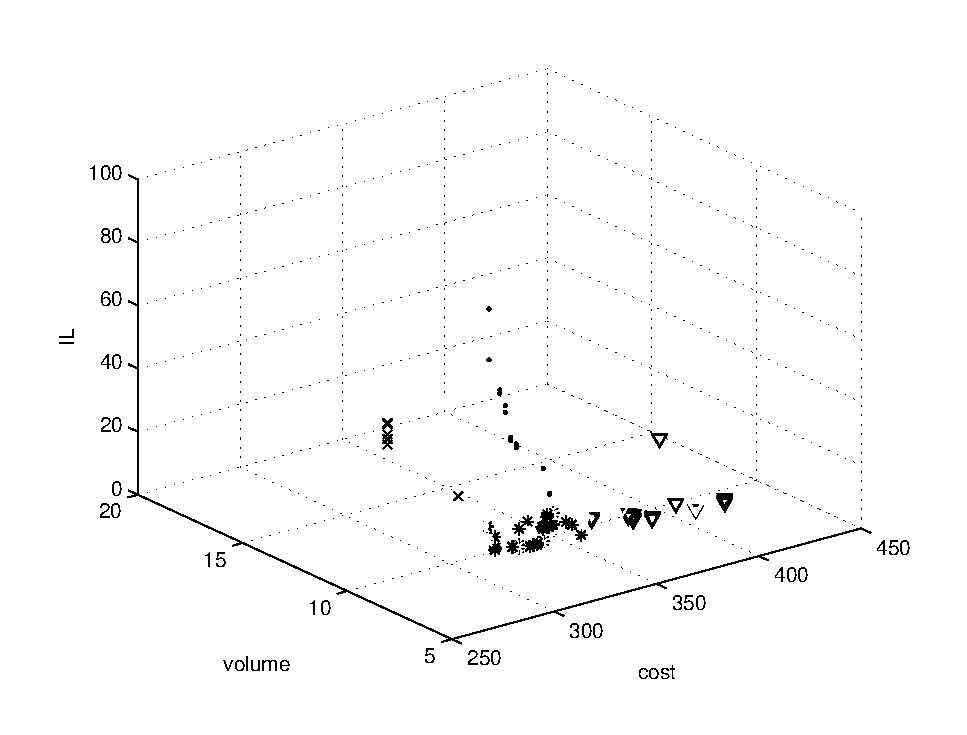
\includegraphics[width=8cm]{ultiplot.eps}
\end{center}
\vspace{-0.5cm}
\caption{3D view (interconnection length-volume-cost) of the Pareto frontier}
\begin{center}
\begin{scriptsize}
$\cdot$ : 1 tier; $\times$ : 2 tiers; + : 3 tiers; * : 4 tiers; $\triangledown$ : 5 tiers
\end{scriptsize}
\end{center}
\label{fig:ds3dview}
\end{figure}

\begin{figure}[h!]
\begin{center}
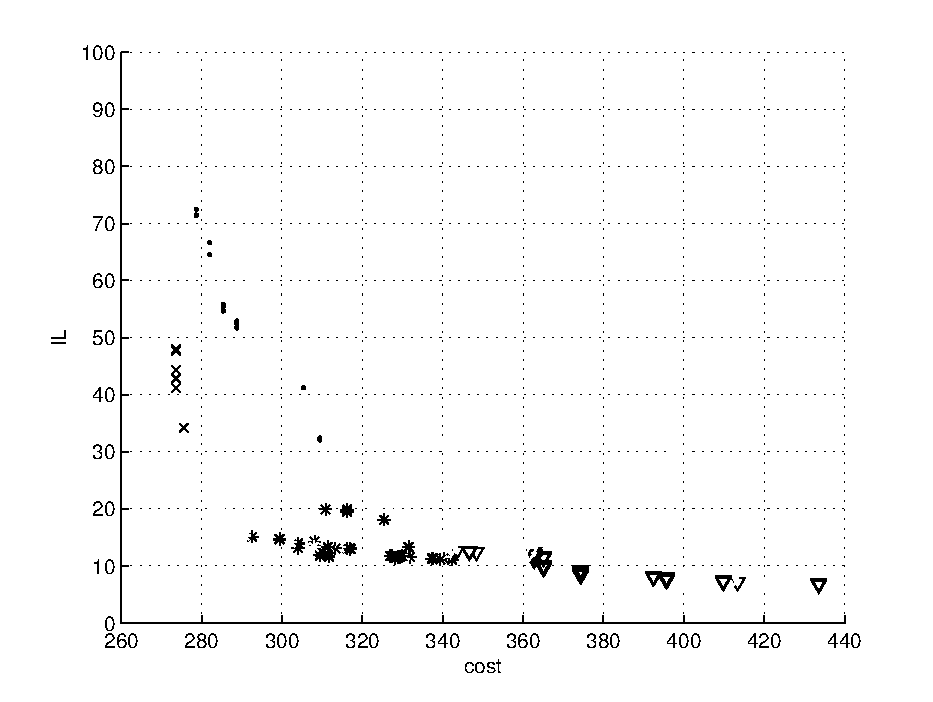
\includegraphics[width=8cm]{ultiplot1.pdf}
\end{center}
\vspace{-0.5cm}
\caption{IL-cost projection view of the Pareto frontier}
\begin{center}
\begin{scriptsize}
$\cdot$ : 1 tier; $\times$ : 2 tiers; + : 3 tiers; * : 4 tiers; $\triangledown$ : 5 tiers\\
\end{scriptsize}
\end{center}
\label{fig:ilcview}
\end{figure}

These results did not take into account the degree of freedom of aspect ratio. If we go further by releasing a degree of freedom and allowing varying aspect ratios, we can have the Pareto front shown in Fig. \ref{fig:ilcview_ff}. This figure shows the Pareto front from Fig. \ref{fig:ilcview} (without aspect ratio, symbol: $\cdot$) alongside with a new Pareto front (with aspect ratio, symbol: +).

As expected, the Pareto front given when considering varying aspect ratios is globally better. Furthermore, by comparing the two graphs, we can see an interesting area where the two frontiers begin to merge at the cost value 350. This means that, in that area, it is not necessary to take the aspect ratio into account. Once again, these kind of information can be important in the design of an IC and yet they would not be available with the current design flows since only a small number of possibilities are explored. Indeed, due to the sequential nature of the current design flows, such degrees of freedom are not even tried since they dramatically increase the duration of each optimization loop.

\begin{figure}[h!]
\begin{center}
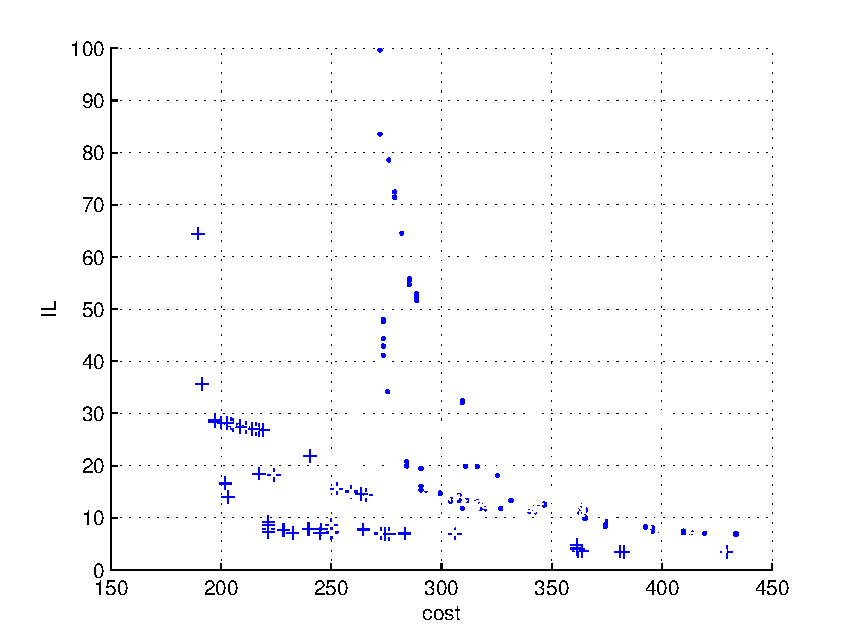
\includegraphics[width=8cm]{ultiplot_ff.pdf}
\end{center}
\vspace{-0.5cm}
\caption{IL-cost projection view of the Pareto frontier (with and without aspect ratio)}
\begin{center}
\begin{scriptsize}
$\cdot$ : Pareto front without aspect ratio; + : Pareto front with aspect ratio\\
\end{scriptsize}
\end{center}
\label{fig:ilcview_ff}
\end{figure}

\section{Validation with a more realist case study}
In the previous section, we have shown how a circuit can be modelled in 3D-SIC to apply a multi-objective optimisation. This case study remains however simple as it contains only 12 blocks. In order to show the applicability of a multi-criteria methodology, we will use a more realist case study. It will still be based on the 3MF platform and we will apply a scale effect where we will consider 12 ADRES processors instead of 6 and also separate the L1 cache memory from each computing unit. We will also add 2 L2 data cache memories and 2 L2 instruction cache memories. This will thus increase the number of working blocks to **. In addition, we will also consider size variability.

\section{Conclusion}

The results have thus shown interesting analyses that can be relevant for a designer. First, using a multi-objective optimization methodology does not only consider all the criteria at the same time but also proceed to an extensive design space exploration which is rarely done with current tools. Second, the qualitative results shown here can give relevant information to the designer and they can be quantified with a more accurate model. Third, the flexibility of MOO allows to easily consider new degrees of freedom without having to change the paradigm. Finally, this methodology and the associated algorithms has shown positive indicators of convergence and robustness as it will be shown in the next chapter.
